\documentclass{standalone}
%\usepackage{amsmath}\usepackage{lmodern}      % Matches the MathJax default (Latin Modern)
%\usepackage[T1]{fontenc}  % Ensures proper character encoding
\usepackage{tikz}
\usetikzlibrary{positioning, arrows.meta, calc}

% Document metadata (Safe to keep in preamble, standalone will skip them during crop)
\title{Chapter 03 — section 04 — diagram 01}
\author{0im}
\date{2026}

\begin{document}
    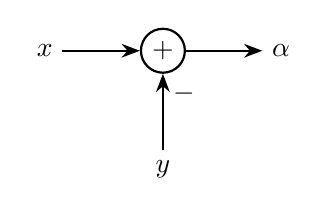
\begin{tikzpicture}
    [
        on grid, 
        node distance=1.5cm and 1.5cm, % Fixed: Added explicit cm units
        block/.style={draw, rectangle, minimum height=2em, minimum width=3em, thick},
        sum/.style={draw, circle, inner sep=2pt, thick},
        branch/.style={draw, circle, inner sep=1.5pt, thick}
    ]
        % =========================================================================
        % NODES
        % =========================================================================
        % --- Row 1 ---
        \node (x) {$x$};
        \node [sum, right=of x] (sum1) {$+$};
        \node [right=of sum1] (alpha) {$\alpha$};
        % --- Row 2 ---
        \node [below=of sum1] (y) {$y$};
        
        % =========================================================================
        % PATHS
        % =========================================================================
        % --- HORIZONTAL ---
        %  Row 1
        \draw [-Stealth, thick] (x) -- (sum1.west);
        \draw [-Stealth, thick] (sum1.east) -- (alpha.west);
        % --- VERTICAL ---
        %  Column 1
        \draw [-Stealth, thick] (y.north) -- (sum1.south)
            node [anchor=north west] {$-$};

    \end{tikzpicture}

\end{document}